\documentclass[]{book}
\usepackage{lmodern}
\usepackage{amssymb,amsmath}
\usepackage{ifxetex,ifluatex}
\usepackage{fixltx2e} % provides \textsubscript
\ifnum 0\ifxetex 1\fi\ifluatex 1\fi=0 % if pdftex
  \usepackage[T1]{fontenc}
  \usepackage[utf8]{inputenc}
\else % if luatex or xelatex
  \ifxetex
    \usepackage{mathspec}
  \else
    \usepackage{fontspec}
  \fi
  \defaultfontfeatures{Ligatures=TeX,Scale=MatchLowercase}
\fi
% use upquote if available, for straight quotes in verbatim environments
\IfFileExists{upquote.sty}{\usepackage{upquote}}{}
% use microtype if available
\IfFileExists{microtype.sty}{%
\usepackage{microtype}
\UseMicrotypeSet[protrusion]{basicmath} % disable protrusion for tt fonts
}{}
\usepackage[margin=1in]{geometry}
\usepackage{hyperref}
\hypersetup{unicode=true,
            pdftitle={Probability and Genetics},
            pdfauthor={Bill Bynum and Brian Avery},
            pdfborder={0 0 0},
            breaklinks=true}
\urlstyle{same}  % don't use monospace font for urls
\usepackage{natbib}
\bibliographystyle{apalike}
\usepackage{color}
\usepackage{fancyvrb}
\newcommand{\VerbBar}{|}
\newcommand{\VERB}{\Verb[commandchars=\\\{\}]}
\DefineVerbatimEnvironment{Highlighting}{Verbatim}{commandchars=\\\{\}}
% Add ',fontsize=\small' for more characters per line
\usepackage{framed}
\definecolor{shadecolor}{RGB}{248,248,248}
\newenvironment{Shaded}{\begin{snugshade}}{\end{snugshade}}
\newcommand{\KeywordTok}[1]{\textcolor[rgb]{0.13,0.29,0.53}{\textbf{#1}}}
\newcommand{\DataTypeTok}[1]{\textcolor[rgb]{0.13,0.29,0.53}{#1}}
\newcommand{\DecValTok}[1]{\textcolor[rgb]{0.00,0.00,0.81}{#1}}
\newcommand{\BaseNTok}[1]{\textcolor[rgb]{0.00,0.00,0.81}{#1}}
\newcommand{\FloatTok}[1]{\textcolor[rgb]{0.00,0.00,0.81}{#1}}
\newcommand{\ConstantTok}[1]{\textcolor[rgb]{0.00,0.00,0.00}{#1}}
\newcommand{\CharTok}[1]{\textcolor[rgb]{0.31,0.60,0.02}{#1}}
\newcommand{\SpecialCharTok}[1]{\textcolor[rgb]{0.00,0.00,0.00}{#1}}
\newcommand{\StringTok}[1]{\textcolor[rgb]{0.31,0.60,0.02}{#1}}
\newcommand{\VerbatimStringTok}[1]{\textcolor[rgb]{0.31,0.60,0.02}{#1}}
\newcommand{\SpecialStringTok}[1]{\textcolor[rgb]{0.31,0.60,0.02}{#1}}
\newcommand{\ImportTok}[1]{#1}
\newcommand{\CommentTok}[1]{\textcolor[rgb]{0.56,0.35,0.01}{\textit{#1}}}
\newcommand{\DocumentationTok}[1]{\textcolor[rgb]{0.56,0.35,0.01}{\textbf{\textit{#1}}}}
\newcommand{\AnnotationTok}[1]{\textcolor[rgb]{0.56,0.35,0.01}{\textbf{\textit{#1}}}}
\newcommand{\CommentVarTok}[1]{\textcolor[rgb]{0.56,0.35,0.01}{\textbf{\textit{#1}}}}
\newcommand{\OtherTok}[1]{\textcolor[rgb]{0.56,0.35,0.01}{#1}}
\newcommand{\FunctionTok}[1]{\textcolor[rgb]{0.00,0.00,0.00}{#1}}
\newcommand{\VariableTok}[1]{\textcolor[rgb]{0.00,0.00,0.00}{#1}}
\newcommand{\ControlFlowTok}[1]{\textcolor[rgb]{0.13,0.29,0.53}{\textbf{#1}}}
\newcommand{\OperatorTok}[1]{\textcolor[rgb]{0.81,0.36,0.00}{\textbf{#1}}}
\newcommand{\BuiltInTok}[1]{#1}
\newcommand{\ExtensionTok}[1]{#1}
\newcommand{\PreprocessorTok}[1]{\textcolor[rgb]{0.56,0.35,0.01}{\textit{#1}}}
\newcommand{\AttributeTok}[1]{\textcolor[rgb]{0.77,0.63,0.00}{#1}}
\newcommand{\RegionMarkerTok}[1]{#1}
\newcommand{\InformationTok}[1]{\textcolor[rgb]{0.56,0.35,0.01}{\textbf{\textit{#1}}}}
\newcommand{\WarningTok}[1]{\textcolor[rgb]{0.56,0.35,0.01}{\textbf{\textit{#1}}}}
\newcommand{\AlertTok}[1]{\textcolor[rgb]{0.94,0.16,0.16}{#1}}
\newcommand{\ErrorTok}[1]{\textcolor[rgb]{0.64,0.00,0.00}{\textbf{#1}}}
\newcommand{\NormalTok}[1]{#1}
\usepackage{longtable,booktabs}
\usepackage{graphicx,grffile}
\makeatletter
\def\maxwidth{\ifdim\Gin@nat@width>\linewidth\linewidth\else\Gin@nat@width\fi}
\def\maxheight{\ifdim\Gin@nat@height>\textheight\textheight\else\Gin@nat@height\fi}
\makeatother
% Scale images if necessary, so that they will not overflow the page
% margins by default, and it is still possible to overwrite the defaults
% using explicit options in \includegraphics[width, height, ...]{}
\setkeys{Gin}{width=\maxwidth,height=\maxheight,keepaspectratio}
\IfFileExists{parskip.sty}{%
\usepackage{parskip}
}{% else
\setlength{\parindent}{0pt}
\setlength{\parskip}{6pt plus 2pt minus 1pt}
}
\setlength{\emergencystretch}{3em}  % prevent overfull lines
\providecommand{\tightlist}{%
  \setlength{\itemsep}{0pt}\setlength{\parskip}{0pt}}
\setcounter{secnumdepth}{5}
% Redefines (sub)paragraphs to behave more like sections
\ifx\paragraph\undefined\else
\let\oldparagraph\paragraph
\renewcommand{\paragraph}[1]{\oldparagraph{#1}\mbox{}}
\fi
\ifx\subparagraph\undefined\else
\let\oldsubparagraph\subparagraph
\renewcommand{\subparagraph}[1]{\oldsubparagraph{#1}\mbox{}}
\fi

%%% Use protect on footnotes to avoid problems with footnotes in titles
\let\rmarkdownfootnote\footnote%
\def\footnote{\protect\rmarkdownfootnote}

%%% Change title format to be more compact
\usepackage{titling}

% Create subtitle command for use in maketitle
\newcommand{\subtitle}[1]{
  \posttitle{
    \begin{center}\large#1\end{center}
    }
}

\setlength{\droptitle}{-2em}
  \title{Probability and Genetics}
  \pretitle{\vspace{\droptitle}\centering\huge}
  \posttitle{\par}
  \author{Bill Bynum and Brian Avery}
  \preauthor{\centering\large\emph}
  \postauthor{\par}
  \predate{\centering\large\emph}
  \postdate{\par}
  \date{2018-01-13}

\usepackage{booktabs}
\usepackage{amsthm}
\makeatletter
\def\thm@space@setup{%
  \thm@preskip=8pt plus 2pt minus 4pt
  \thm@postskip=\thm@preskip
}
\makeatother

\usepackage{amsthm}
\newtheorem{theorem}{Theorem}[chapter]
\newtheorem{lemma}{Lemma}[chapter]
\theoremstyle{definition}
\newtheorem{definition}{Definition}[chapter]
\newtheorem{corollary}{Corollary}[chapter]
\newtheorem{proposition}{Proposition}[chapter]
\theoremstyle{definition}
\newtheorem{example}{Example}[chapter]
\theoremstyle{definition}
\newtheorem{exercise}{Exercise}[chapter]
\theoremstyle{remark}
\newtheorem*{remark}{Remark}
\newtheorem*{solution}{Solution}
\begin{document}
\maketitle

{
\setcounter{tocdepth}{1}
\tableofcontents
}
\chapter*{Preface}\label{preface}
\addcontentsline{toc}{chapter}{Preface}

\section{Motivation}\label{motivation}

\section{About the Authors}\label{about-the-authors}

\chapter{Coin flips and Chromosomes - Probability Basics and Tree
Diagrams}\label{basics}

\section{Introduction}\label{introduction}

In this chapter, basic terminology and principles of probability are
introduced along with simulation and tree diagrams as important tools to
analyze probability questions.

\section{Chapter Scenario}\label{chapter_scenario}

Imagine a simple situation where two coins are tossed and the number of
heads is observed and the outcome has some relevance for you depending
on whether the result yields 0, 1, or 2 heads. Do you think each of
these outcomes is equally likely? What do you think is the probability
of each of these outcomes?

We use this coin-flipping scenario as a primary example not because we
have inherent interest flipping coins but because this scenario is an
effective model for many real-world situations such as gene inheritance.

\section{Terminology}\label{terminology}

\textbf{Probability} is the measure of the likelihood of an event on a
scale of 0 to 1 where a probability of 1 can be interpreted as certainty
the event will occur and a probability of 0 interpreted as certainty the
event will NOT occur. There are two main schools of thought regarding
what probability is - the frequentist and the bayesian - but for our
initial purposes we will think of the probability of an event as the
relative frequency of its occurrence in the long run. In very informal
shorthand, we think of probability as the ratio of successes to the
total number of trials as shown below but must be careful to distinguish
between exact theoretical probabilities and approximate empirical
probabilities.

\[Probability = \frac{successes}{total}\]

Consider a coin is flipped and we examine whether it lands on heads or
tails. We say it is a fair coin if heads and tails are equally likely.
In this case, the probability of the coin landing on heads is \(1/2\)
which can also be expressed as \(0.5\) or \(50\%\) meaning that as the
experiment is repeated the proportion of heads ultimately approaches
0.50. It does not mean that in any number of trials we will obtain heads
exactly \(50\%\) of the time as samples will vary.

A \textbf{probability experiment} is a process with a random element
producing a well-defined outcome such as the tossing of a coin described
above and the chapter scenario described above where two coins are
flipped and you are interested in whether 0, 1, or 2 heads are seen. An
\textbf{event} is any well-defined outcome of the probability
experiment, such as, the outcome of getting at least one head when
flipping two coins.

We often use function notation when describing probabilities. For event
\textbf{E} in a probability experiment we will use \textbf{P(E)} to
represent the probability event E occurs. We also informally use short
descriptions of events combined with probability function notation. For
example, when flipping one coin we can note \(P(heads)=1/2\).

The \textbf{sample space} is a list of all possible outcomes of a
probability experiment. One desirable property of a sample space
description is that the simple events we use are \textbf{equally
likely}, meaning all have the same probability of occurring. For
example, for the experiment of flipping two coins one might consider
\(\{0\,heads,\,1\, head,\,2\,heads\}\) as a potential sample space but
enquiring minds might wonder whether or not each of these outcomes is
equally likely.

\section{Simulation}\label{simulation}

Simulation is often a helpful tool to explore probability questions like
the question above regarding whether getting 0, 1, or 2 heads when
flipping two coins are all equally likely. The code below simulates
10,000 trials of two coin flips keeping track of the number of heads,
number of tails, and proportion of heads for each trial.

\begin{Shaded}
\begin{Highlighting}[]
\NormalTok{sim_}\DecValTok{2}\NormalTok{ <-}\StringTok{ }\KeywordTok{do}\NormalTok{(}\DecValTok{10000}\NormalTok{)}\OperatorTok{*}\KeywordTok{rflip}\NormalTok{(}\DataTypeTok{n=}\DecValTok{2}\NormalTok{, }\DataTypeTok{prob=}\DecValTok{1}\OperatorTok{/}\DecValTok{2}\NormalTok{)}
\NormalTok{knitr}\OperatorTok{::}\KeywordTok{kable}\NormalTok{(}
  \KeywordTok{head}\NormalTok{(sim_}\DecValTok{2}\NormalTok{), }\DataTypeTok{caption =} \StringTok{'Table 1: Two Coin Simulation'}\NormalTok{,}
  \DataTypeTok{booktabs =} \OtherTok{TRUE}
\NormalTok{)}
\end{Highlighting}
\end{Shaded}

\begin{table}

\caption{\label{tab:nice-tab}Table 1: Two Coin Simulation}
\centering
\begin{tabular}[t]{rrrr}
\toprule
n & heads & tails & prop\\
\midrule
2 & 0 & 2 & 0.0\\
2 & 0 & 2 & 0.0\\
2 & 1 & 1 & 0.5\\
2 & 2 & 0 & 1.0\\
2 & 1 & 1 & 0.5\\
2 & 2 & 0 & 1.0\\
\bottomrule
\end{tabular}
\end{table}

The result is visualized in a histogram of the \texttt{heads} variable
showing the frequency of obtaining 0, 1, and 2 heads.

\begin{Shaded}
\begin{Highlighting}[]
\KeywordTok{ggplot}\NormalTok{(}\DataTypeTok{data=}\NormalTok{sim_}\DecValTok{2}\NormalTok{, }\KeywordTok{aes}\NormalTok{(}\DataTypeTok{x=}\NormalTok{heads)) }\OperatorTok{+}\StringTok{ }\KeywordTok{geom_histogram}\NormalTok{(}\KeywordTok{aes}\NormalTok{(}\DataTypeTok{y=}\NormalTok{..density..), }\DataTypeTok{binwidth =} \DecValTok{1}\NormalTok{)}
\end{Highlighting}
\end{Shaded}

\begin{figure}

{\centering 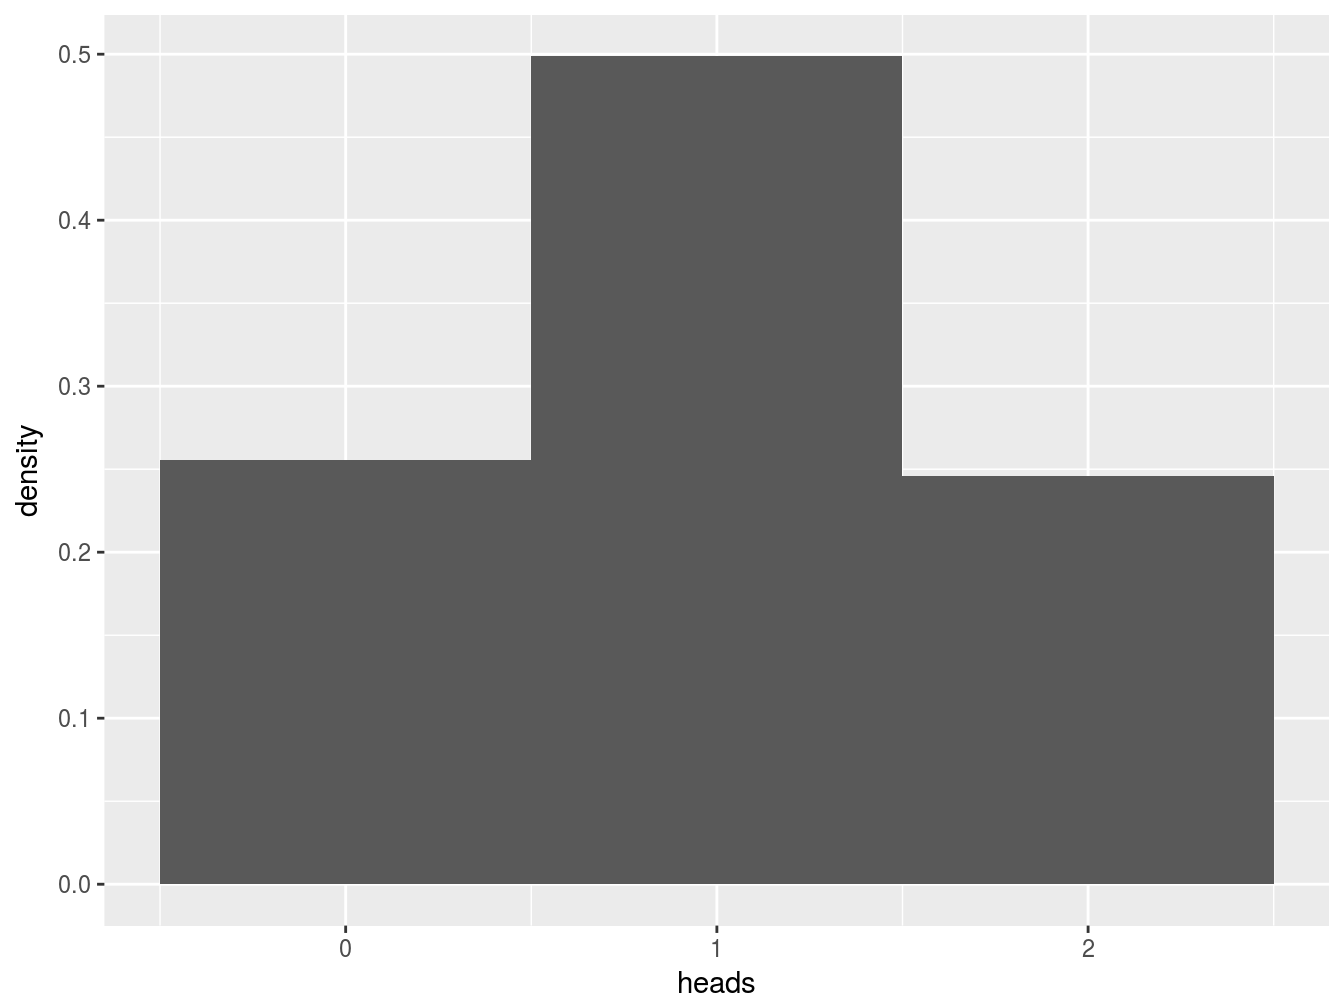
\includegraphics[width=0.8\linewidth]{probgen-bookdown_files/figure-latex/nice-fig-1-1} 

}

\caption{Histogram for Number of Heads When Flipping Two Coins}\label{fig:nice-fig-1}
\end{figure}

Examining the histogram we see that obtaining one head is more likely
than the other two options and, thus, getting 0, 1, and 2 heads when
flipping two coins are not equally likely outcomes. Prompted by the
results of the simulation, we want to know why getting one head is more
likely and tree diagrams will help us.

\section{Tree Diagrams}\label{tree_diagrams}

The outcomes of a probability experiment can be catalogued with a tree
diagram where at each node the different branches represent the
different possible outcomes at each stage of the process.

Consider the tree diagram for flipping a single coin where we label each
node as either H for Heads or T for tails and label the probability
along each branch.

\begin{figure}

{\centering 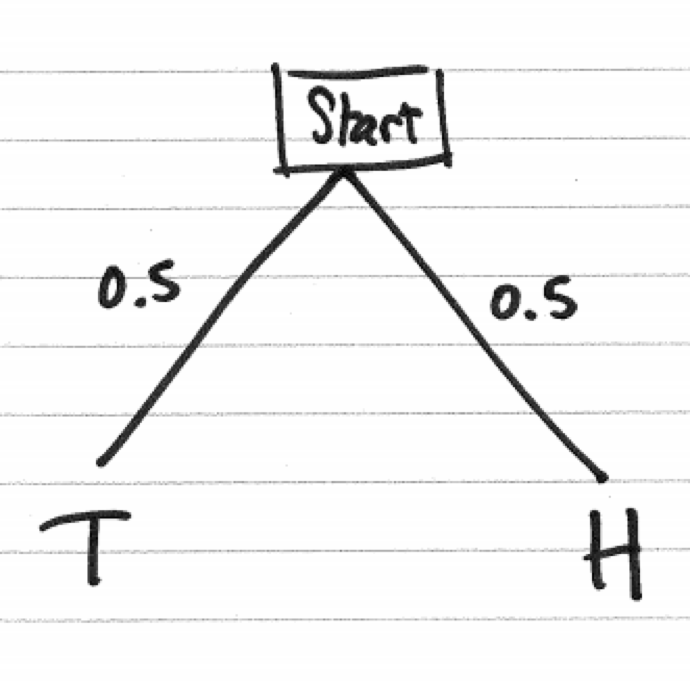
\includegraphics[width=0.3\linewidth]{01-basics-figures/tree_one_coin} 

}

\caption{Tree Diagram for One Coin}\label{fig:nice-fig-2}
\end{figure}

Including the possible outcomes for a second coin results in a tree
diagram with four branches.

\begin{figure}

{\centering 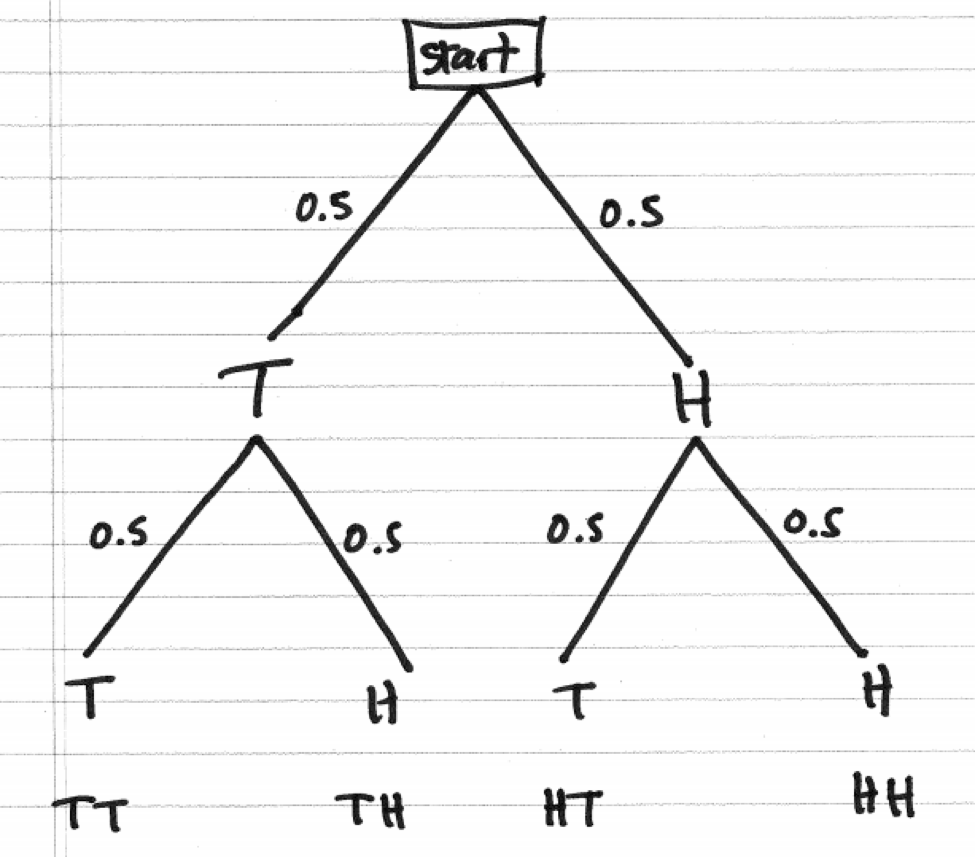
\includegraphics[width=0.6\linewidth]{01-basics-figures/tree_two_coins} 

}

\caption{Tree Diagram for Two Coins}\label{fig:nice-fig-3}
\end{figure}

Each path from the top of the tree to the bottom represents one possible
outcome when tossing two coins. In this experiment, there is a 50/50
chance of getting heads or tails thus all four paths are equally likely
each occurring with probability \(0.5 \times 0.5 = 0.25\). If we think
of the probability associated with each branch as the proportion of the
time we travel down that branch then multiplying these probabilities
makes perfect sense to determine the probability of traveling down
sequential branches.

We can now understand why getting one head is more likely as there are
two paths, HT and TH, compared to only one path generating zero heads,
TT, and only one path generating two heads, HH, resulting in the
following probabilities:

\[P(0\ heads) = P(TT) = (0.5)(0.5) = 0.25\]
\[\small P(1\ head) = P(TH\ or\ HT) = P(TH) + P(HT) = (0.5)(0.5) + (0.5)(0.5) = 0.25 + 0.25 = 0.5\]

\[P(2\ heads) = P(HH) = (0.5)(0.5) = 0.25\]

\subsection{An Example with Rats}\label{an_example_with_rats}

Now consider the experiment of choosing three rats at random from a
large population of rats that is 40\% male and 60\% female. Just as we
did for coins, we can draw a tree diagram with branches representing the
sex of the first, second, and third rat chosen and label the associated
probabilities on each branch. Selecting the rats and identifying gender
would be equivalent to having a coin that lands on one side 40\% of the
time and on the other 60\% of the time. In the tree diagram below, we
have added subscripts to identify whether we are referring to the first,
second, or third rat selected.

\begin{figure}

{\centering 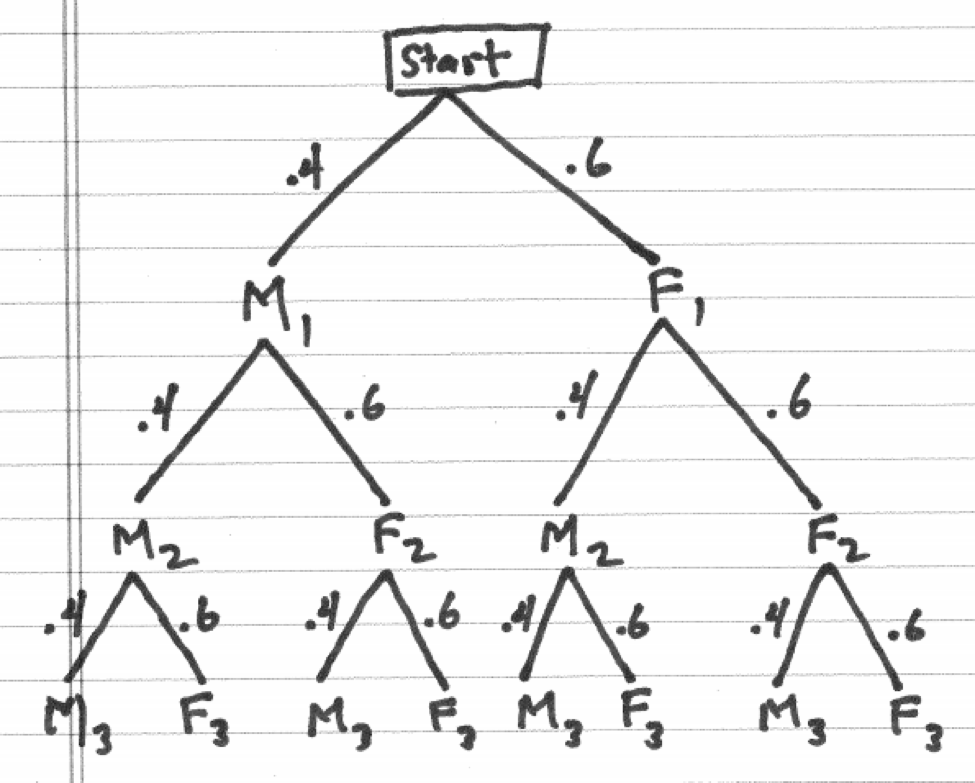
\includegraphics[width=0.6\linewidth]{01-basics-figures/tree_rat_sex} 

}

\caption{Tree Diagram for Three Rats}\label{fig:nice-fig-4}
\end{figure}

What is the probability of selecting 0 female rats? Note that because
the population is large at each stage of the process the probability of
selecting a female rat is 0.60.

\[P(0\ female\ rats) = P(M_{1}\ and\ M_{2}\ and\ M_{3}) = (0.4) \times (0.4) \times (0.4) = 0.064\]

What is the probability of selecting 1 female rat? There are actually
three distinct paths through the tree where 1 female rat and 2 male rats
are selected and each one has the probability \((0.6) \times (0.4)^2\)
thus the probability is

\[P(1\ female\ rat) = 3 \times (0.6) (0.4)^2 = 0.288\]

\subsubsection{Practice Exercise 1}\label{practice-exercise-1}

For the probability experiment described above choosing three rats at
random from a large population of rats that is 40\% male and 60\%
female, what is the probability of getting 2 female rats? 3 female rats?

\subsubsection{Practice Exercise 2}\label{practice-exercise-2}

Draw a tree diagram for the probability experiment of flipping three
coins. Label each node as either H for Heads or T for tails and label
the probability along each branch. Find the probabilities of obtaining
exactly 0 heads, 1 head, 2 heads, and 3 heads.

\section{The Urn Model}\label{the_urn_model}

When confronted with a question of personal importance to you where
probabilistic concerns are relevant to getting an accurate answer, the
ability to develop a model that captures important probability details
is a key problem-solving tool. By \textbf{model} we mean a systematic
description that shares all of the important characterics of the
problem, be it a physical, visual, mathematical, or computational
representation (\url{http://www.dictionary.com/browse/model}).

For probability experiments two useful models are the coin-flipping
model and the urn model. We have already looked briefly at a
coin-flipping experiment. We will see throughout our probabilistic
treatment of genetics that we will often use coin-flipping as a mental
model to think about questions of genetic risk and reward. The urn model
is another important way to think about probability questions.

Consider an urn with some beads in it. Imagine the urn has 20 beads 12
of which are black and 8 white and we are to draw out three of these
beads at random and we want to find the probability of ending up with 0,
1, 2, or 3 black beads.

\begin{figure}

{\centering 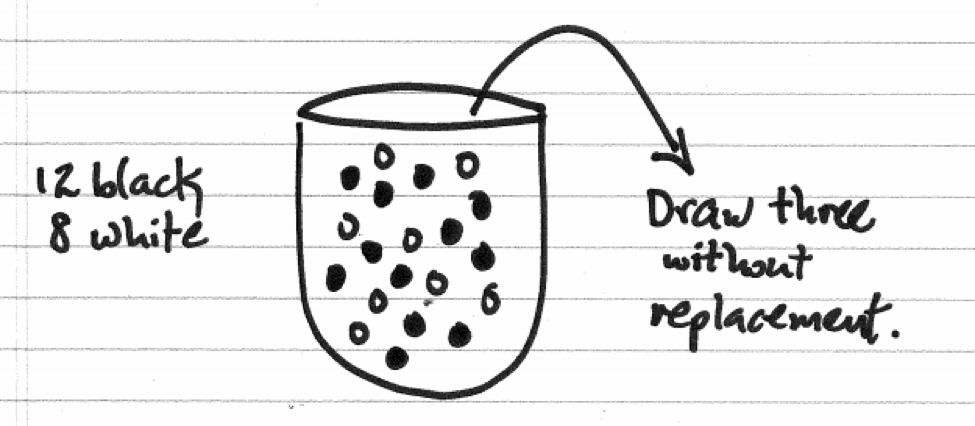
\includegraphics[width=0.6\linewidth]{01-basics-figures/urn1_picture} 

}

\caption{The Urn Model}\label{fig:nice-fig-5}
\end{figure}

First, we need to be clear up one question: is the drawing out of beads
to be done with replacement or without replacement? By \textbf{with
replacement} we mean that after each draw of one bead, it is replaced,
the beads thoroughly mixed, before another bead is selected at random.
By \textbf{without replacement} we mean that after one bead is removed,
it is not replaced before the next bead is selected. Note, if we are
selecting three beads at once this could be viewed as equivalent to
selecting the beads one at a time without replacement.

\begin{figure}

{\centering 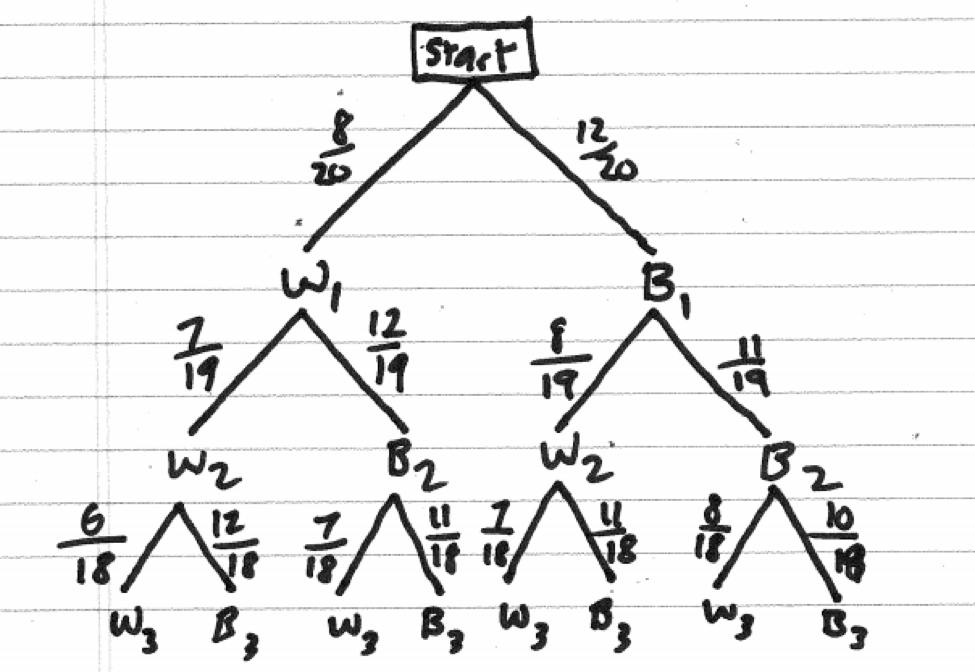
\includegraphics[width=0.6\linewidth]{01-basics-figures/tree_urn1} 

}

\caption{Tree Diagram for Three Beads}\label{fig:nice-fig-6}
\end{figure}

For this experiment with three beads drawn at random without replacement
from an urn containing 12 black and 8 white beads, what is the
probability of ending up with 0, 1, 2, or 3 black beads, respectively?

First, let's tackle the probability of getting 0 black beads. From
examining the tree we see

\[P(0\ blacks) = P(W_{1}\ and\ W_{2}\ and\ W_{3}) = \frac{8}{20} \times \frac{7}{19} \times \frac{6}{18}\]

Finding the probability of one black is more work. As we examine the
tree we see there are three distinct paths resulting in one black. Check
out their separate probabilities here.

\[P(B_{1}\ and\ W_{2}\ and\ W_{3}) = \frac{12}{20} \times \frac{8}{19} \times \frac{7}{18} = 0.098\]

\[P(W_{1}\ and\ B_{2}\ and\ W_{3}) = \frac{8}{20} \times \frac{12}{19} \times \frac{7}{18} = 0.098\]

\[P(W_{1}\ and\ W_{2}\ and\ B_{3}) = \frac{8}{20} \times \frac{7}{19} \times \frac{12}{18} = 0.098\]

In spite of the numerators being in different orders, we notice that
these three separate probabilities are numerically equal. Thus, for the
final probability we see

\[P(1\ black) = 3 \times \frac{12}{20} \times \frac{8}{19} \times \frac{7}{18} = 0.295\]

\section{Ands, Ors, and Nots}\label{and_ors_nots}

Most of the interesting probability questions involve combinations of
simple events. In this section we examine the probabilities of two
events both occurring (\textbf{and}), at least one of two events
occurring (\textbf{or}), as well as an event not occurring
(\textbf{not}).

\subsection{In an Attempt to Kill the Student, the Authors Solve the
Same Simple Problem Four Ways (One Bad and Three
Good)}\label{kill_the_student}

By dissecting an easy problem we can gain insight into multiple
problem-solving strategies that can be useful in other problems. Or we
can kill motivation altogether. We will see.

In the game of Risk competitors resolve attacks by rolling dice. Suppose
that you are rolling two dice and you are interested in whether or not
we obtain a six. We consider the following compound events.

While there are six sides to each die, because we are primarily
interested in whether or not we obtain a six, we will use the tree
diagram below where event \textbf{S} represents getting a six and event
\textbf{N} represents getting a non-six, ie., 1, 2, 3, 4, or 5.

\begin{figure}

{\centering 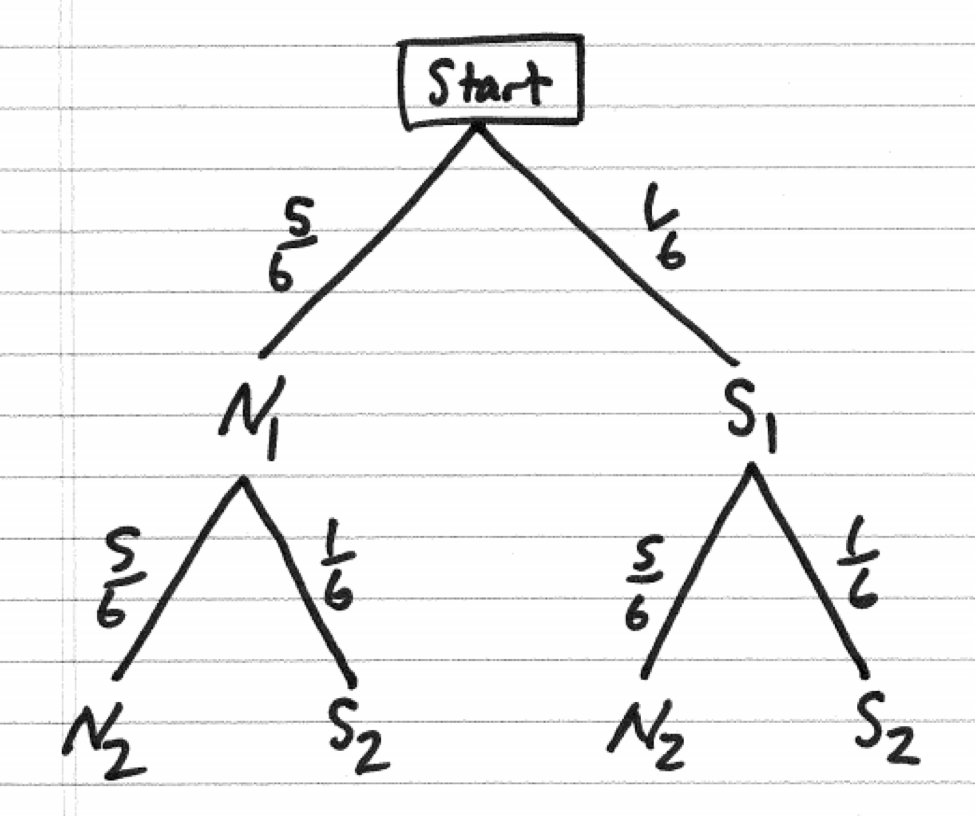
\includegraphics[width=0.6\linewidth]{01-basics-figures/tree_two_dice_sixes} 

}

\caption{Tree Diagram for Sixes on Two Dice}\label{fig:nice-fig-7}
\end{figure}

Even if we are tossing identical dice simultaneously it is helpful to
conceptualize the experiment as if we are tossing the dice sequentially.
We have added subscripts to identify whether we are referring to the
first die tossed or the second die tossed.

What is the probability of obtaining a six on both dice? Because the two
events of getting a six on the first die and getting a six on the second
die are \textbf{independent}, we can use \textbf{The Multiplication Rule
for Independent Events} which says for any two independent events \(E\)
and \(F\), \(P(E\ and\ F) = P(E) \times P(F)\).

\[P(two\ sixes) = P(S_{1}\ and\ S_{2}) = P(S_{1}) \times P(S_{2}) =  \frac{1}{6} \times \frac{1}{6}\]

What is the probability of obtaining a six on at least one of the two
dice? We examine this problem from four points of view - the wrong point
of view, the addition rule, the partition technique, and the complement
principle.

\subsubsection{The Wrong Way}\label{the-wrong-way}

Here is a faulty answer:

\[P(at\ least\ one\ six) = P(S_{1}\ or\ S_{2}) = P(S_{1})+ P(S_{2}) = \frac{1}{6} + \frac{1}{6} = \frac{2}{6} = \frac{1}{3}\ \ WRONG!\]

Can you spot the problem? The issue is that one branch with a six on
both dice, the overlap where both events \(S_{1}\) and \(S_{2}\) occur,
was counted twice.

\subsubsection{The Addition Rule}\label{the-addition-rule}

Here is a correct version using what is called \textbf{The Addition
Rule} where the overlap, since it was counted twice, is subtracted:

\[P(at\ least\ one\ six) = P(S_{1}\ or\ S_{2}) = P(S_{1})+ P(S_{2}) - P(S_{1}\ AND\ S_{2}) =\\ \frac{1}{6} + \frac{1}{6} - \frac{1}{6} \times \frac{1}{6}  = \frac{11}{36}\]

\subsubsection{The Partition Approach}\label{the-partition-approach}

An alternative approach is to \textbf{partition} the event into mutually
exclusive parts. We might informally describe this approach as
\emph{divide and conquer}. In this case, there are three distinct
branches that satisfy at least one six occurring:

\[P(at\ least\ one\ six) = P(S_{1}\ and\ N_{2}) + P(N_{1}\ and\ S_{2}) + P(S_{1}\ and\ S_{2}) = \\  \frac{1}{6} \times \frac{5}{6} + \frac{5}{6} \times \frac{1}{6} + \frac{1}{6} \times \frac{1}{6} = \frac{11}{36}\]

\subsubsection{The Complement Principle}\label{the-complement-principle}

A third correct approach uses \textbf{The Complement Principle} which
observes that for any event \(E\), \(P(E) = 1 - P(not\ E)\). In this
situation, we note \(P(at\ least\ one) = 1 - P(none)\). Sometimes it is
less work to find the complement of an event and subtract from one.

\[P(at\ least\ one\ six) = 1 - P(no\ sixes) = 1 - P(N_{1}\ and\ N_{2}) = \\  1 - \frac{5}{6} \times \frac{5}{6} = \frac{11}{36}\]

To summarize what we have learned about problem-solving here, there is
more than one way to solve a probability problem (and some ways are
wrong!). But several good strategies to use are the addition rule being
careful not to double-count, divide and conquer by partitioning the
event into mutually exclusive pieces, or use the complement principle to
solve the opposite problem and subtract this from one.

\section{Appendix 1: Genetics
Examples}\label{appendix-1-genetics-examples}

In this appendix, you are introduced to the absolute basic terminology
of genetics and how the principles of probability that you learned in
chapter 1 can be applied to genetics.\\
We are going to adapt the examples from the main part of chapter 1 to
genetics. We'll look at some of the same tree diagrams and simulations
but within a simple genetics framework (rather than coin flips and
urns).

\subsection{Genetics Terminology}\label{genetics-terminology}

For now, we are going to use the minimum of genetic lingo to get going:

\textbf{trait}: a characteristic, something you can see or measure
(e.g.~height, Huntington's disease)

\textbf{gene}: the DNA that controls a trait (e.g.~hemoglobin beta gene)
usually shown with a letter or letters (e.g.~Hb)

\textbf{variant}: one of several versions of a gene (e.g.~HbS variant in
hemoglobin beta that can cause Sickle Cell Anemia but there are other
variants of the same gene (HbC, HbE, etc.), a.k.a. allele)

\textbf{chromosome}: long, continuous stretch of DNA that contains many
genes (humans have 2 copies of each of 22 numbered chromosomes and
either 2 X chromosomes for females or an X and a Y for males)

\textbf{gamete}: specialized cell that has only 1 copy of each
chromosome that is used during sexual reproduction (e.g.~egg or sperm)

\subsection{Genetics Basics}\label{genetics-basics}

\subsubsection{intro to chromosomal
genetics}\label{intro-to-chromosomal-genetics}

\begin{itemize}
\tightlist
\item
  humans have 2 copies of every gene (can be same variant or different)
\item
  \textbf{meiosis} is the process of making gametes with only 1 copy of
  all of the genes
\item
  \textbf{fertilization} fuses two gametes each with 1 copy back into a
  cell/organism with 2 copies (1 from each parent/gamete)
\end{itemize}

To summarize the important points about \textbf{meiosis}, parents each
make gametes that contain only one of their 2 possible copies of each
chromosome. Then the gametes can fuse together by fertilization to make
the offspring (next generation) that again has 2 copies of each
chromosome (one from each of their parents).

Below are some cartoons of meiosis starting with an example cell that
has 2 chromosomes (one with the A gene and a second with the B gene) and
this organism has 2 copies of each chromosome.

\begin{figure}

{\centering 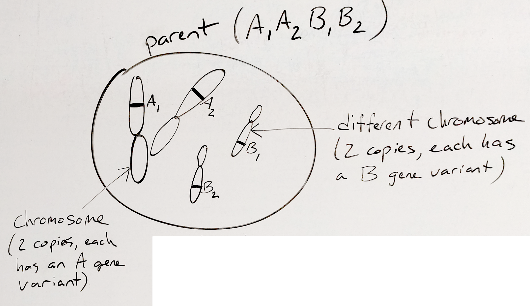
\includegraphics[width=0.75\linewidth]{01-basics-figures/meiosis1} 

}

\caption{cartoon example cell}\label{fig:gen-fig-1}
\end{figure}

Notice that the chromosomes have different variants.

When that cell goes through meiosis, it produces gametes that have one
copy of each of the 2 different chromosomes.

\begin{figure}

{\centering 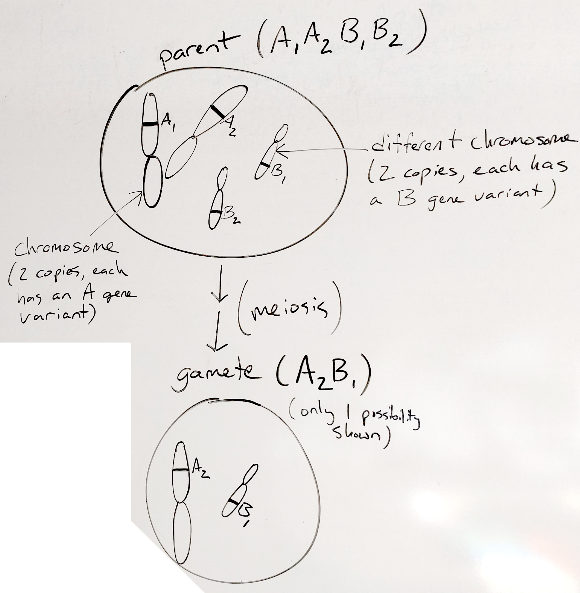
\includegraphics[width=0.75\linewidth]{01-basics-figures/meiosis2} 

}

\caption{making gametes}\label{fig:gen-fig-2}
\end{figure}

Compare the original/parent and gamete and convince yourself that this
gamete has one of each of the different chromosomes in the
original/parent organism. Notice that the figure below says that the
gamete shown is only one of the possibilities. If you like to think
ahead, what are the other possibilities? If you're not up for it yet,
don't worry, we'll get there.

To make an offspring, 2 gametes fuse by fertilization.

\begin{figure}

{\centering 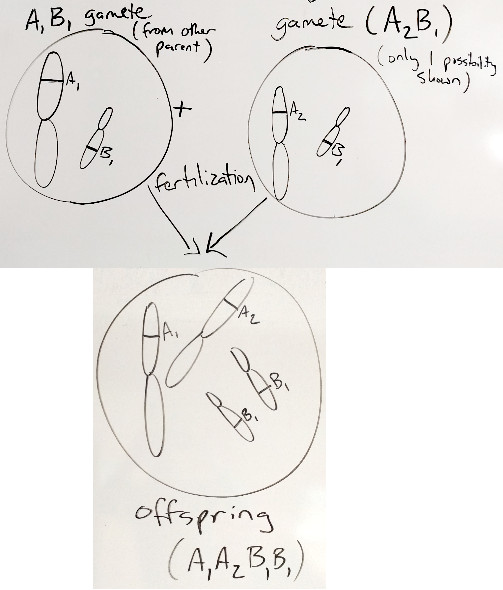
\includegraphics[width=0.75\linewidth]{01-basics-figures/meiosis3} 

}

\caption{fertilization}\label{fig:gen-fig-3}
\end{figure}

Since each gamete has only 1 copy of each chromosome, when 2 gametes
fuse, there are again 2 copies of each chromosome (one from each of
their parents). So, new humans have 2 chromosomes, one from each parent.

\subsubsection{thinking
probilitisically}\label{thinking-probilitisically}

To wrap this back around to probability and tree diagrams, you can think
of each parent as having a coin for each chromosome, and each
chromosome-coin has 2 sides - H and T for a coin, one for each copy of
the chromosome (A1 or A2). The chromosome version is equally likely to
fall on the A1 or A2 ``side'' (as long as we only consider one gene on
each chromosome, which we will do for now). So, our tree diagram looks
like this:

\begin{figure}

{\centering 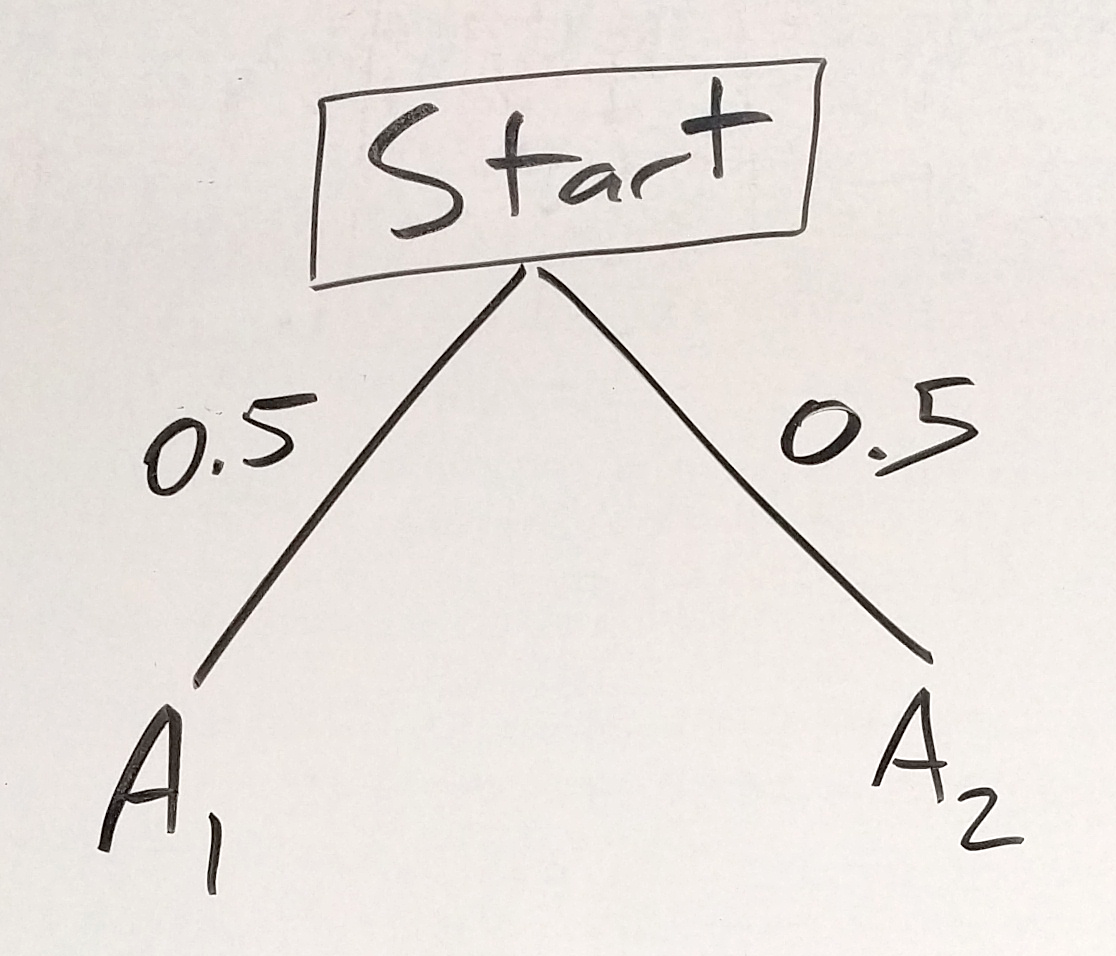
\includegraphics[width=0.5\linewidth]{01-basics-figures/1csome_tree} 

}

\caption{one chromosome tree - first parent}\label{fig:gen-fig-4}
\end{figure}

Now if we think of the gametes from the second parent as a second
``coin'' with A1 and A2 ``sides'', our tree diagram looks like this:

\begin{figure}

{\centering \includegraphics[width=0.7\linewidth]{01-basics-figures/1csome_tree2} 

}

\caption{one chromosome tree - second parent}\label{fig:gen-fig-5}
\end{figure}

Then we can use the multiplication rule to find the probabilities of the
different offspring as seen below:

\begin{figure}

{\centering \includegraphics[width=0.9\linewidth]{01-basics-figures/1csome_tree3} 

}

\caption{one chromosome tree - offspring}\label{fig:gen-fig-6}
\end{figure}

We can also use the addition rule to clean up our prediction a bit since
most of the time it doesn't matter which parent you get an allele from,
so A1A2 and A2A1 are equivalent and we can add their probabilities
together to get a combined \(p(A1A2)=0.5\).

Also notice that in the tree diagrams and in parentheses in the meiosis
drawings that we often just write the gene/variant shorthand. This
shorthand is called the \textbf{genotype} and is pretty useful since it
can save you from drawing a lot of chromosomes, but if you need the
chromosomes to be sure you understand what's going on, feel free to
sketch away.

\subsubsection{intro to DNA}\label{intro-to-dna}

There are 4 main DNA letters (a.k.a. \emph{bases}) - A, T, C, G - that
make up genes, which can be thought of as DNA ``words''. While it's not
my favorite analogy, it works reasonably well - genes are collections of
DNA information. There are variants (different versions) of genes that
change the letters, and many of those change the information the gene
contains, and can change the organism.

\subsubsection{\texorpdfstring{genetic
``notation''}{genetic notation}}\label{genetic-notation}

Geneticists (a lot like mathematicians) use abbreviations as short cuts
a lot. They are first introduced above in the \emph{Genetics
Terminology} section, and again discussed at the end of the
\emph{Thinking Probabilistically} section but we'll lay it out more
here.

Every gene has an abbreviated name (like a nickname) that makes it
easier to write. For example, the hemoglobin beta gene goes by
\textbf{Hb}. We use that as a base, then we add other letters to modify
this name to show that we are talking about specific variants like the
\textbf{HbS} variant in hemoglobin beta that can cause sickle cell
anemia. Just to break that down, the \textbf{Hb} part tells us the gene,
and the \textbf{S} part tells us which variant.

Sometimes we will use numbers, such as A1 and A2 to mean the 1 and 2
variants of the A gene, or for other genes we'll use lowercase and
uppercase, such as B and b, to mean different variants of the same gene.

And as a review, writing just the letter shorthand for all of the genes
and variants together is the \textbf{genotype} of an organism.

\subsection{Genetics Simulation}\label{genetics-simulation}

Now we'll use R to simulate the same situation shown in the tree diagram
above. This version takes the long way around, but it conceptually
models meiosis (gamete formation) and fertilization for 1000 offspring.

Our first set of parents have the genotypes below:\\
parent 1: A1/A1\\
parent 2: A2/A2

The code below simulates meiosis and fertilization of 1000 offspring,
makes a table, and graphs the results.

\begin{Shaded}
\begin{Highlighting}[]
\CommentTok{# set up the different variants that each parent has}
\NormalTok{parent1_variants <-}\StringTok{ }\KeywordTok{c}\NormalTok{(}\StringTok{'A1'}\NormalTok{,}\StringTok{'A1'}\NormalTok{)}
\NormalTok{parent2_variants <-}\StringTok{ }\KeywordTok{c}\NormalTok{(}\StringTok{'A2'}\NormalTok{,}\StringTok{'A2'}\NormalTok{)}

\CommentTok{# list of 1000 gametes from each parent, probability of each is equal by default}
\NormalTok{parent1_gametes <-}\StringTok{ }\KeywordTok{sample}\NormalTok{(parent1_variants, }\DecValTok{1000}\NormalTok{, }\DataTypeTok{replace =} \OtherTok{TRUE}\NormalTok{)}
\NormalTok{parent2_gametes <-}\StringTok{ }\KeywordTok{sample}\NormalTok{(parent2_variants, }\DecValTok{1000}\NormalTok{, }\DataTypeTok{replace =} \OtherTok{TRUE}\NormalTok{)}

\CommentTok{# put gametes together to make 1000 offspring}
\NormalTok{cross_x1 <-}\StringTok{ }\KeywordTok{paste}\NormalTok{(parent1_gametes, parent2_gametes, }\DataTypeTok{sep=}\StringTok{"/"}\NormalTok{)}
\NormalTok{offspring1 <-}\StringTok{ }\KeywordTok{data.frame}\NormalTok{(}\KeywordTok{table}\NormalTok{(cross_x1))}

\CommentTok{# table}
\NormalTok{knitr}\OperatorTok{::}\KeywordTok{kable}\NormalTok{(offspring1, }\DataTypeTok{caption =} \StringTok{'A1xA2 parent cross simulation'}\NormalTok{, }\DataTypeTok{booktabs =} \OtherTok{TRUE}\NormalTok{)}
\end{Highlighting}
\end{Shaded}

\begin{table}

\caption{\label{tab:unnamed-chunk-3}A1xA2 parent cross simulation}
\centering
\begin{tabular}[t]{lr}
\toprule
cross\_x1 & Freq\\
\midrule
A1/A2 & 1000\\
\bottomrule
\end{tabular}
\end{table}

\begin{Shaded}
\begin{Highlighting}[]
\CommentTok{# makes a bar graph of the frequency of genotypes}
\KeywordTok{ggplot}\NormalTok{(offspring1, }\KeywordTok{aes}\NormalTok{(}\DataTypeTok{x=}\NormalTok{cross_x1, }\DataTypeTok{y=}\NormalTok{Freq)) }\OperatorTok{+}\StringTok{ }\KeywordTok{geom_bar}\NormalTok{(}\DataTypeTok{stat=}\StringTok{"identity"}\NormalTok{)}
\end{Highlighting}
\end{Shaded}

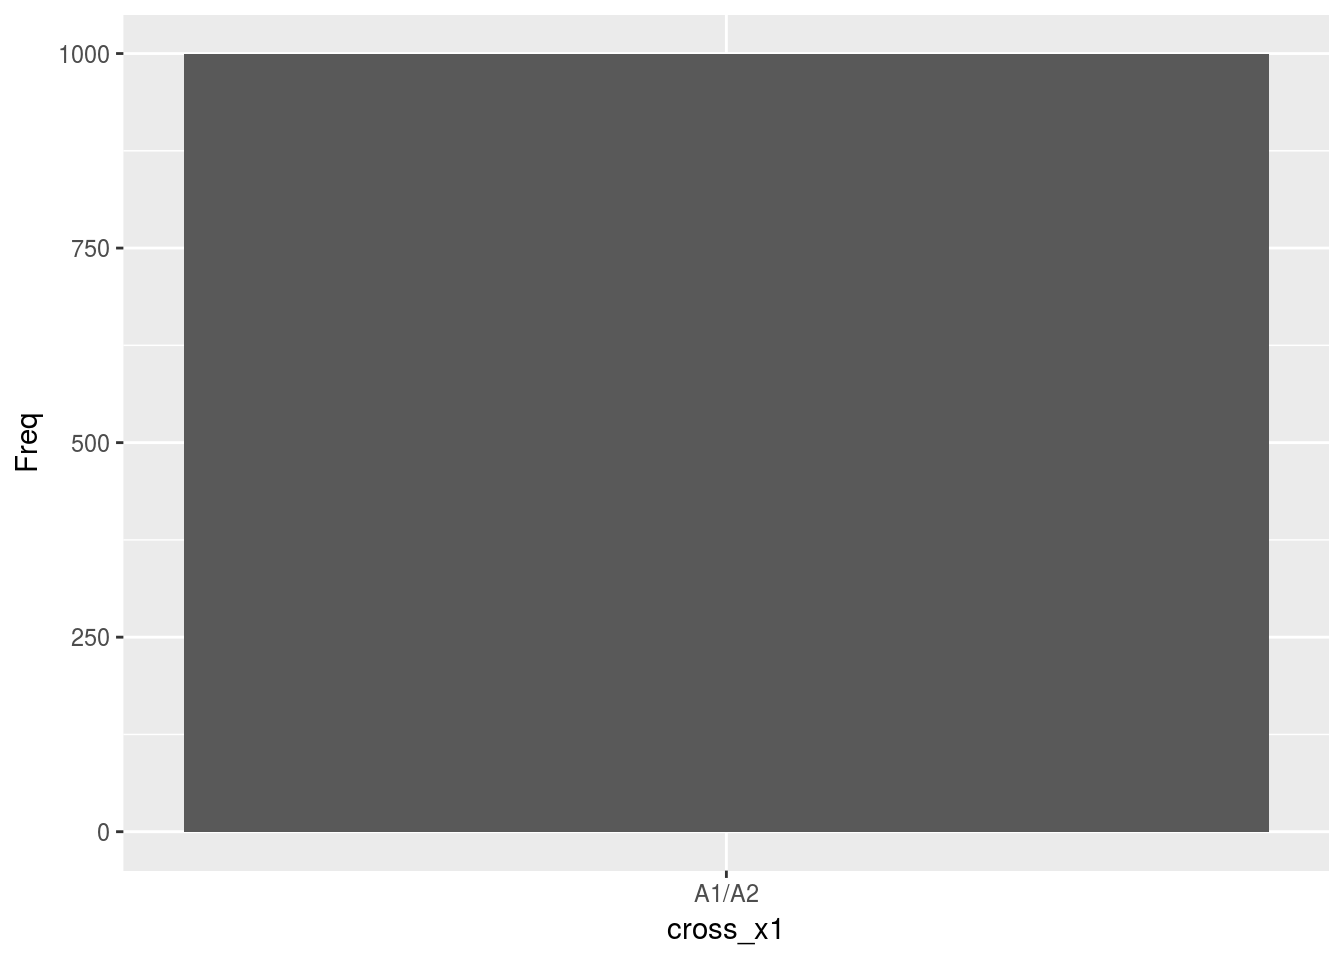
\includegraphics{probgen-bookdown_files/figure-latex/unnamed-chunk-3-1.pdf}

Now that we have the results for that set of offspring (all have the
A1/A2 genotype), we can look at these offspring as parents for a new
generation of offspring. Now the parents are:\\
parent 1: A1/A2\\
parent 2: A1/A2

The code below simulates meiosis and fertilization of 1000 offspring,
makes a table, and graphs the results.

\begin{Shaded}
\begin{Highlighting}[]
\CommentTok{# set up the different variants that each parent has}
\NormalTok{parent3_variants <-}\StringTok{ }\KeywordTok{c}\NormalTok{(}\StringTok{'A1'}\NormalTok{,}\StringTok{'A2'}\NormalTok{)}
\NormalTok{parent4_variants <-}\StringTok{ }\KeywordTok{c}\NormalTok{(}\StringTok{'A1'}\NormalTok{,}\StringTok{'A2'}\NormalTok{)}

\CommentTok{# list of 1000 gametes from each parent, probability of each is equal by default}
\NormalTok{parent3_gametes <-}\StringTok{ }\KeywordTok{sample}\NormalTok{(parent3_variants, }\DecValTok{1000}\NormalTok{, }\DataTypeTok{replace =} \OtherTok{TRUE}\NormalTok{)}
\NormalTok{parent4_gametes <-}\StringTok{ }\KeywordTok{sample}\NormalTok{(parent4_variants, }\DecValTok{1000}\NormalTok{, }\DataTypeTok{replace =} \OtherTok{TRUE}\NormalTok{)}

\CommentTok{# put gametes together to make 1000 offspring}
\NormalTok{cross_x2 <-}\StringTok{ }\KeywordTok{paste}\NormalTok{(parent3_gametes, parent4_gametes, }\DataTypeTok{sep=}\StringTok{"/"}\NormalTok{)}
\NormalTok{cross_x2 <-}\StringTok{ }\KeywordTok{gsub}\NormalTok{(}\StringTok{"A2/A1"}\NormalTok{, }\StringTok{"A1/A2"}\NormalTok{, cross_x2) }\CommentTok{# order doesn't matter}
\NormalTok{offspring2 <-}\StringTok{ }\KeywordTok{data.frame}\NormalTok{(}\KeywordTok{table}\NormalTok{(cross_x2))}

\CommentTok{# table}
\NormalTok{knitr}\OperatorTok{::}\KeywordTok{kable}\NormalTok{(offspring2, }\DataTypeTok{caption =} \StringTok{'A1/A2 inter-cross simulation'}\NormalTok{, }\DataTypeTok{booktabs =} \OtherTok{TRUE}\NormalTok{)}
\end{Highlighting}
\end{Shaded}

\begin{table}

\caption{\label{tab:unnamed-chunk-4}A1/A2 inter-cross simulation}
\centering
\begin{tabular}[t]{lr}
\toprule
cross\_x2 & Freq\\
\midrule
A1/A1 & 253\\
A1/A2 & 495\\
A2/A2 & 252\\
\bottomrule
\end{tabular}
\end{table}

\begin{Shaded}
\begin{Highlighting}[]
\CommentTok{# makes a bar graph of the frequency of genotypes}
\KeywordTok{ggplot}\NormalTok{(offspring2, }\KeywordTok{aes}\NormalTok{(}\DataTypeTok{x=}\NormalTok{cross_x2, }\DataTypeTok{y=}\NormalTok{Freq)) }\OperatorTok{+}\StringTok{ }\KeywordTok{geom_bar}\NormalTok{(}\DataTypeTok{stat=}\StringTok{"identity"}\NormalTok{)}
\end{Highlighting}
\end{Shaded}

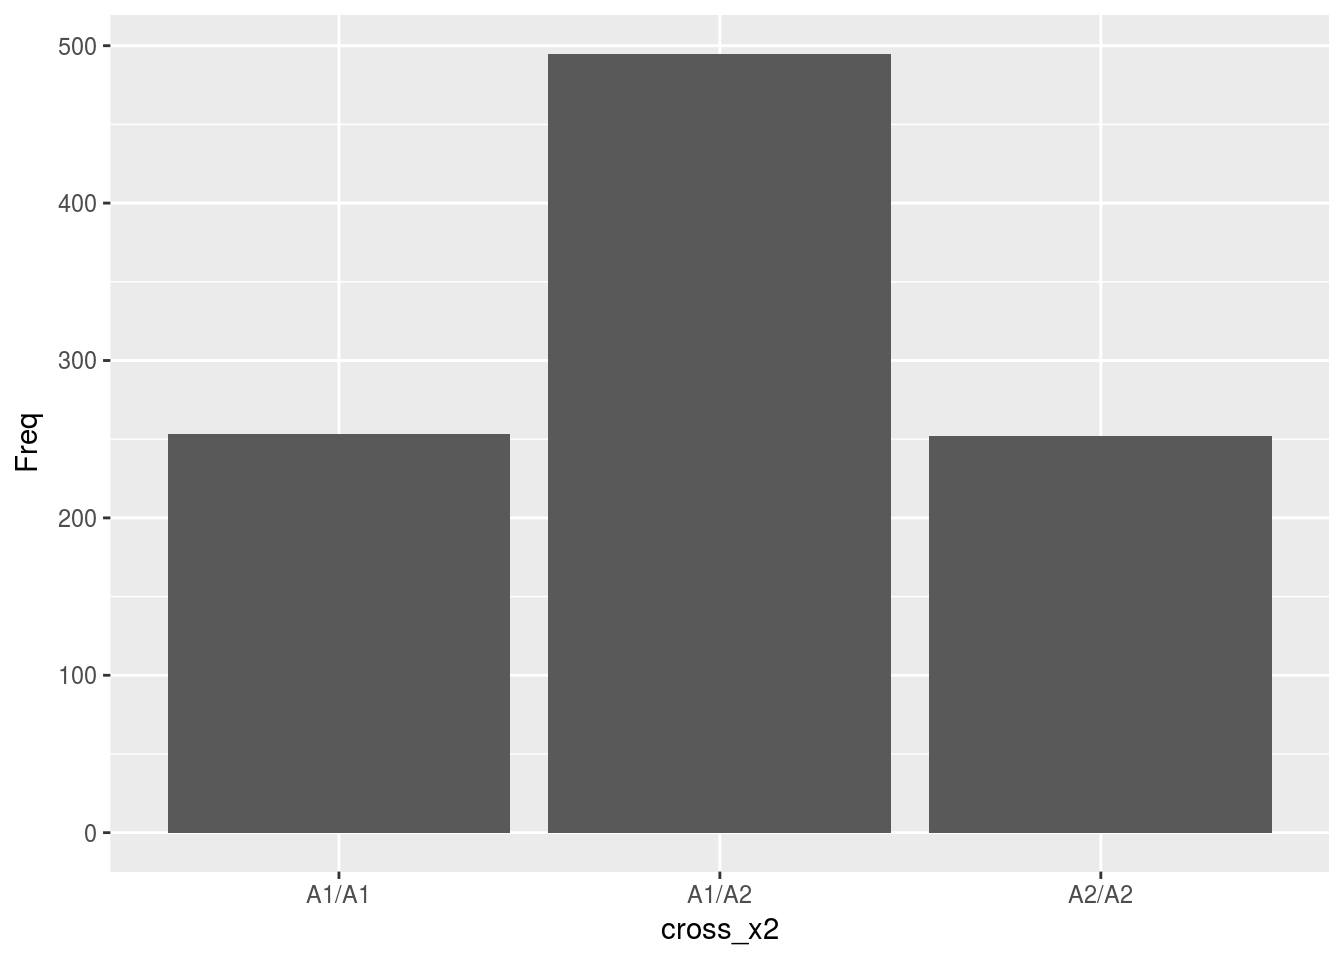
\includegraphics{probgen-bookdown_files/figure-latex/unnamed-chunk-4-1.pdf}

How does this compare to our predicted probabilities from the tree
diagram?\\
Remember that they were:\\
\(p(A1/A1) = 0.25\)\\
\(p(A1/A2) = 0.5\)\\
\(p(A2/A2) = 0.25\)

Should be reasonably close.

Just as an additional example, the same code adapted to use B and b
variants of the B gene:

\begin{Shaded}
\begin{Highlighting}[]
\NormalTok{parent1_variants <-}\StringTok{ }\KeywordTok{c}\NormalTok{(}\StringTok{'B'}\NormalTok{,}\StringTok{'B'}\NormalTok{)}
\NormalTok{parent2_variants <-}\StringTok{ }\KeywordTok{c}\NormalTok{(}\StringTok{'b'}\NormalTok{,}\StringTok{'b'}\NormalTok{)}

\NormalTok{parent1_gametes <-}\StringTok{ }\KeywordTok{sample}\NormalTok{(parent1_variants, }\DecValTok{1000}\NormalTok{, }\DataTypeTok{replace =} \OtherTok{TRUE}\NormalTok{)}
\NormalTok{parent2_gametes <-}\StringTok{ }\KeywordTok{sample}\NormalTok{(parent2_variants, }\DecValTok{1000}\NormalTok{, }\DataTypeTok{replace =} \OtherTok{TRUE}\NormalTok{)}

\NormalTok{cross_x1 <-}\StringTok{ }\KeywordTok{paste}\NormalTok{(parent1_gametes, parent2_gametes, }\DataTypeTok{sep=}\StringTok{""}\NormalTok{)}

\NormalTok{offspring1 <-}\StringTok{ }\KeywordTok{data.frame}\NormalTok{(}\KeywordTok{table}\NormalTok{(cross_x1))}
\NormalTok{knitr}\OperatorTok{::}\KeywordTok{kable}\NormalTok{(offspring1, }\DataTypeTok{caption =} \StringTok{'BBxbb parent cross simulation'}\NormalTok{, }\DataTypeTok{booktabs =} \OtherTok{TRUE}\NormalTok{)}
\end{Highlighting}
\end{Shaded}

\begin{table}

\caption{\label{tab:unnamed-chunk-5}BBxbb parent cross simulation}
\centering
\begin{tabular}[t]{lr}
\toprule
cross\_x1 & Freq\\
\midrule
Bb & 1000\\
\bottomrule
\end{tabular}
\end{table}

\begin{Shaded}
\begin{Highlighting}[]
\KeywordTok{ggplot}\NormalTok{(offspring1, }\KeywordTok{aes}\NormalTok{(}\DataTypeTok{x=}\NormalTok{cross_x1, }\DataTypeTok{y=}\NormalTok{Freq)) }\OperatorTok{+}\StringTok{ }\KeywordTok{geom_bar}\NormalTok{(}\DataTypeTok{stat=}\StringTok{"identity"}\NormalTok{)}
\end{Highlighting}
\end{Shaded}

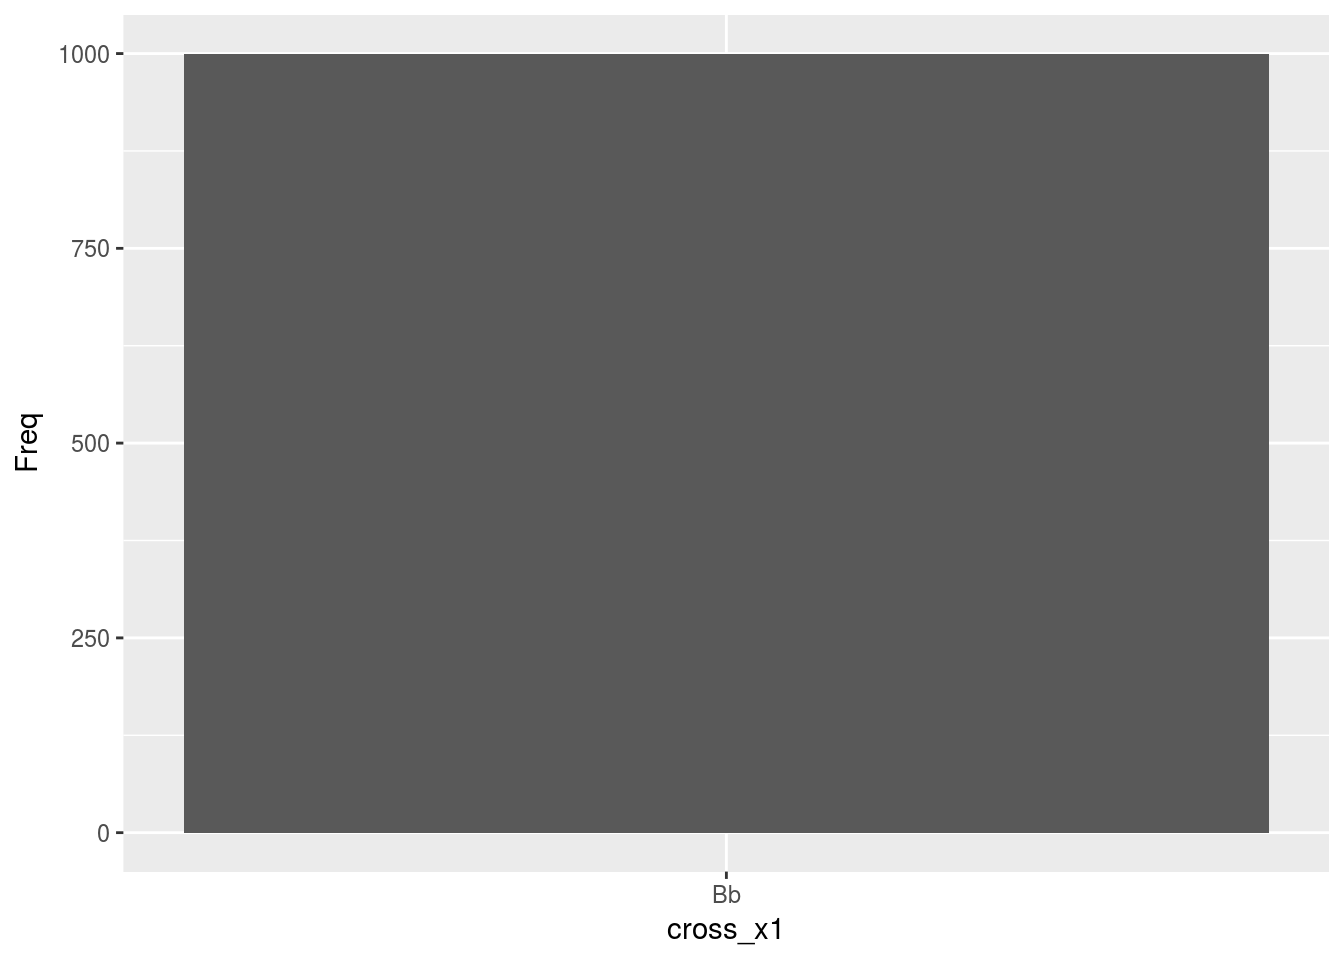
\includegraphics{probgen-bookdown_files/figure-latex/unnamed-chunk-5-1.pdf}

Now intercross the offspring from the first cross, each is Bb:

\begin{Shaded}
\begin{Highlighting}[]
\NormalTok{parent3_variants <-}\StringTok{ }\KeywordTok{c}\NormalTok{(}\StringTok{'B'}\NormalTok{,}\StringTok{'b'}\NormalTok{)}
\NormalTok{parent4_variants <-}\StringTok{ }\KeywordTok{c}\NormalTok{(}\StringTok{'B'}\NormalTok{,}\StringTok{'b'}\NormalTok{)}

\NormalTok{parent3_gametes <-}\StringTok{ }\KeywordTok{sample}\NormalTok{(parent3_variants, }\DecValTok{1000}\NormalTok{, }\DataTypeTok{replace =} \OtherTok{TRUE}\NormalTok{)}
\NormalTok{parent4_gametes <-}\StringTok{ }\KeywordTok{sample}\NormalTok{(parent4_variants, }\DecValTok{1000}\NormalTok{, }\DataTypeTok{replace =} \OtherTok{TRUE}\NormalTok{)}

\NormalTok{cross_x2 <-}\StringTok{ }\KeywordTok{paste}\NormalTok{(parent3_gametes, parent4_gametes, }\DataTypeTok{sep=}\StringTok{""}\NormalTok{)}
\NormalTok{cross_x2 <-}\StringTok{ }\KeywordTok{gsub}\NormalTok{(}\StringTok{"bB"}\NormalTok{, }\StringTok{"Bb"}\NormalTok{, cross_x2)}
\NormalTok{offspring2 <-}\StringTok{ }\KeywordTok{data.frame}\NormalTok{(}\KeywordTok{table}\NormalTok{(cross_x2))}
\NormalTok{knitr}\OperatorTok{::}\KeywordTok{kable}\NormalTok{(offspring2, }\DataTypeTok{caption =} \StringTok{'Bb inter-cross simulation'}\NormalTok{, }\DataTypeTok{booktabs =} \OtherTok{TRUE}\NormalTok{)}
\end{Highlighting}
\end{Shaded}

\begin{table}

\caption{\label{tab:unnamed-chunk-6}Bb inter-cross simulation}
\centering
\begin{tabular}[t]{lr}
\toprule
cross\_x2 & Freq\\
\midrule
bb & 239\\
Bb & 506\\
BB & 255\\
\bottomrule
\end{tabular}
\end{table}

\begin{Shaded}
\begin{Highlighting}[]
\KeywordTok{ggplot}\NormalTok{(offspring2, }\KeywordTok{aes}\NormalTok{(}\DataTypeTok{x=}\NormalTok{cross_x2, }\DataTypeTok{y=}\NormalTok{Freq)) }\OperatorTok{+}\StringTok{ }\KeywordTok{geom_bar}\NormalTok{(}\DataTypeTok{stat=}\StringTok{"identity"}\NormalTok{)}
\end{Highlighting}
\end{Shaded}

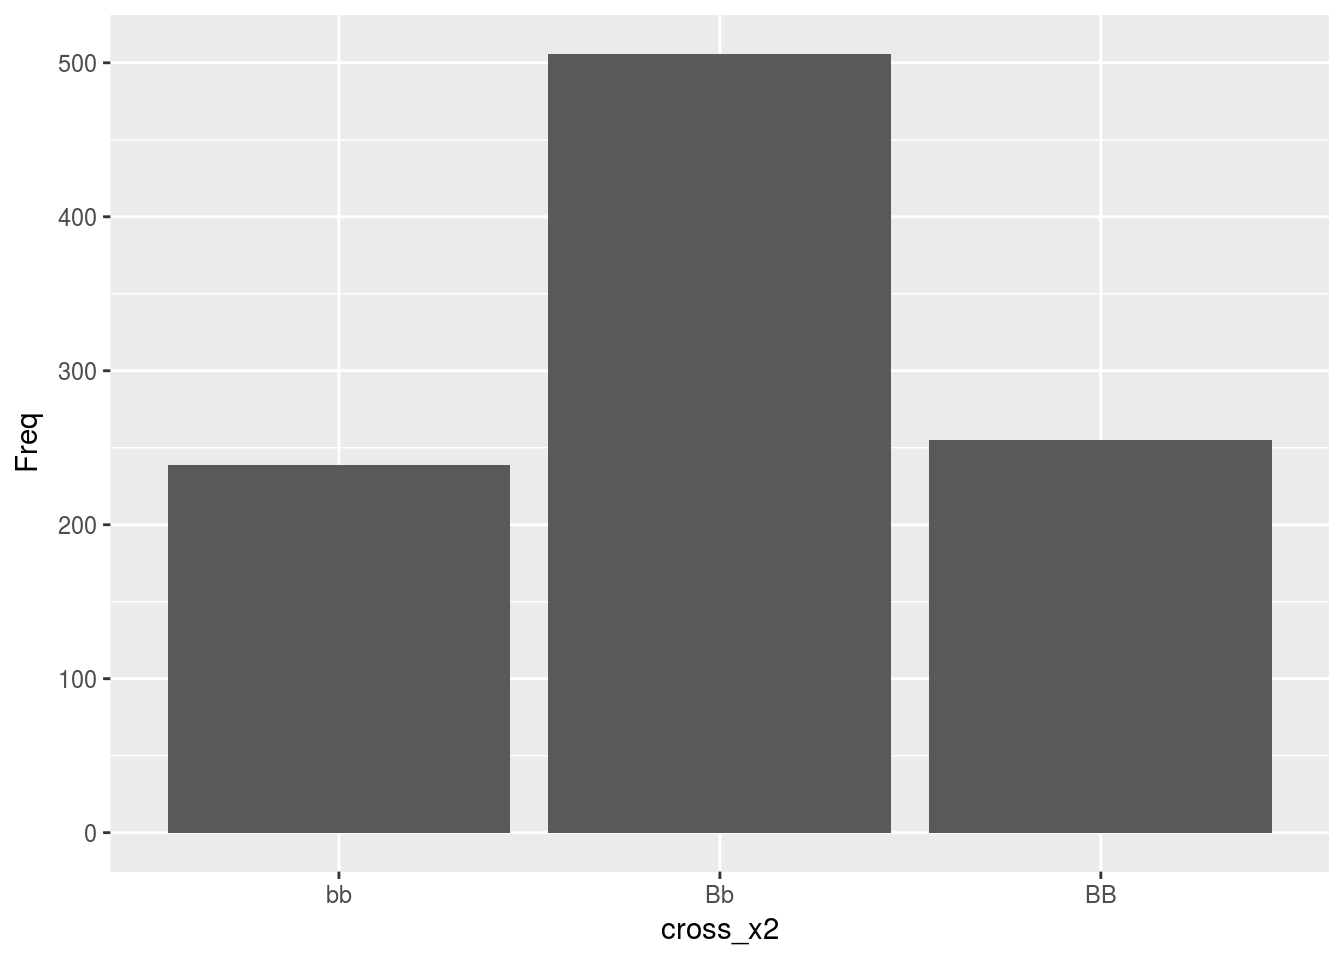
\includegraphics{probgen-bookdown_files/figure-latex/unnamed-chunk-6-1.pdf}

\chapter{Tree Diagrams}\label{trees}

Tree diagrams are very useful for probability.

\chapter{And/Or}\label{and-or}

Logic with \texttt{and} and \texttt{or}\ldots{}

\section{\texorpdfstring{\texttt{and}
statements}{and statements}}\label{and-statements}

\section{\texorpdfstring{\texttt{or}
statements}{or statements}}\label{or-statements}

\chapter{Conditional Probability}\label{conditional}

Conditional probability is a thing.

\section{Example one}\label{example-one}

some stuff

\section{Example two}\label{example-two}

more stuff

\chapter{The Binomial Distribution}\label{the-binomial-distribution}

We describe some cool stuff about the Binomial Distribution in this
chapter.

\chapter{Combinations and
Permutations}\label{combinations-and-permutations}

Combinations and Permutations

\section{Combinations}\label{combinations}

\section{Permutations}\label{permutations}

\chapter{Normal Distribution}\label{normal}

Not everything is Normal (we certainly aren't), but it's useful!

\chapter{Multinomial Distribution}\label{multinom}

Beyond the Binomial to the Multinomial\ldots{}

\chapter{Fancier Distributions}\label{fancy}

Oooh, fancy!

\chapter{Bayes Theorem}\label{bayes}

Probability can give you (apparent) superpowers!

\bibliography{packages.bib,book.bib}


\end{document}
